
\graphicspath{{./chap3/images/}} 
\chapter{Command}
\textbf{이 장은 기본 리눅스 명령어를 다룬다.}
\section{파일 관리}
\subsection{절대경로와 상대경로}
절대경로는 /home/gs19000/dir1/dir2와 같은 것이다. 상대경로는 현재 내 위치에서 시작하는 경로다. 즉, 내가 지금 /home/gs19000/dir1에 있다면 여기서 /home/gs19000/dir1/dir2의 상대경로는 그냥 dir2다.
\subsection{디렉토리 및 탐색}
cd 명령어를 사용해서 디렉터리를 탐색할 수 있다. \\ ..은 상위 디렉토리, -은 이전 디렉토리, $\sim$는 홈 디렉토리를 의미한다.
cd (디렉토리)라 치면 해당 디렉토리로 이동된다. 디렉토리를 표현할 때 절대경로, 상대경로 둘 다 가능하며, 실행시 주소쪽 값이 변경된다.
\begin{lstlisting}
    $ cd dir1 입력시
    ~/dir1$ __으로 바뀐다.
    $ cd /home/gs19000/dir1 
    $ cd ..
    $ cd -
    $ cd ~
\end{lstlisting}
\subsection{디렉토리 및 파일 관리}
rm 명령어를 사용해서 파일을 삭제할 수 있다.\\
rm (file) : 해당 파일을 삭제한다. rm -r (dir) : 해당 디렉토리를 삭제한다.
또한, mkdir 명령어를 사용해서 디렉터리를 만들 수 있다.\\
mkdir (dir) : 해당 이름의 디렉토리가 존재하지 않을 경우 새로 dir이름의 디렉터리를 생성한다.\\


다음으로 cp, mv 명령어를 통해 파일을 옯기거나 복사할 수 있다.\\
cp (file1) (file2) : file1의 이름을 file2 이름으로 바꾸어 복사한다.(file1은 삭제되지 않음 file2가 이미 존재할 경우 덮어씌워진다)\\
cp -r (dir1) (dir2) : dir1이름의 디렉토리를 dir2 디렉토리 내부에 복사한다.(dir1은 반드시 존재해야 하며 dir2는 존재하지 않을 경우 새로 만들어진다)\\
mv (file1) (file2) : file1의 이름을 file2로 바꾼다.(file2가 이미 존재할 경우 덮어씌워진다)\\
mv (dir1) (dir2) : dir1의 이름을 dir2로 바꾼다.(dir1은 반드시 존재해야 하며 dir2가 존재할 경우 dir2 내부에 dir1 파일을 이동시킨다.)\\
마지막으로, cat을 이용해 내용을 읽어올 수 있다. cat (file1) : file1의 내용을 불러온다.
    \begin{lstlisting}
    $ rm file1
    $ rm -r dir1
    $ mkdir dir2
    $ cp file1 file2
    $ cp -r dir1 dir2
    $ mv file1 file2
    $ mv dir1 dir2
    $ cat file3.txt
    \end{lstlisting}
\section{기타 기능}
\subsection{프로세스 관리}
htop을 이용해 실행중인 프로세스를 확인할 수 있다. kill, pkill을 통해 프로세스를 제거할 수 있다.
    \begin{lstlisting}
    $ htop
    $ kill -9 <pid>
    \end{lstlisting}
\subsection{권한 관리}
chmod를 이용해 권한을 관리할 수 있다. 권한에 대한 자세한 정보는 ...
    \begin{lstlisting}
    $ sudo chmod 777 file1
    \end{lstlisting}
\subsection{Vim}
기본 메모장과 같다. 우분투 서버를 지속적으로 다룰 생각이 있다면 Vim 에디터에 익숙해질 필요가 있다. 먼저, vim 에디터를 사용하여 파일을 수정하기 위해서는 vim 에디터를 실행해야 한다. vim 에디터는 다음과 같은 명령어를 통해 실행할 수 있다.
    \begin{lstlisting}
    $ vim filename
    \end{lstlisting}
위와 같이 vim 에디터를 통해 파일을 열게 되면 다음과 같은 화면이 나타난다.

\begin{figure}[H]
	\begin{center}
        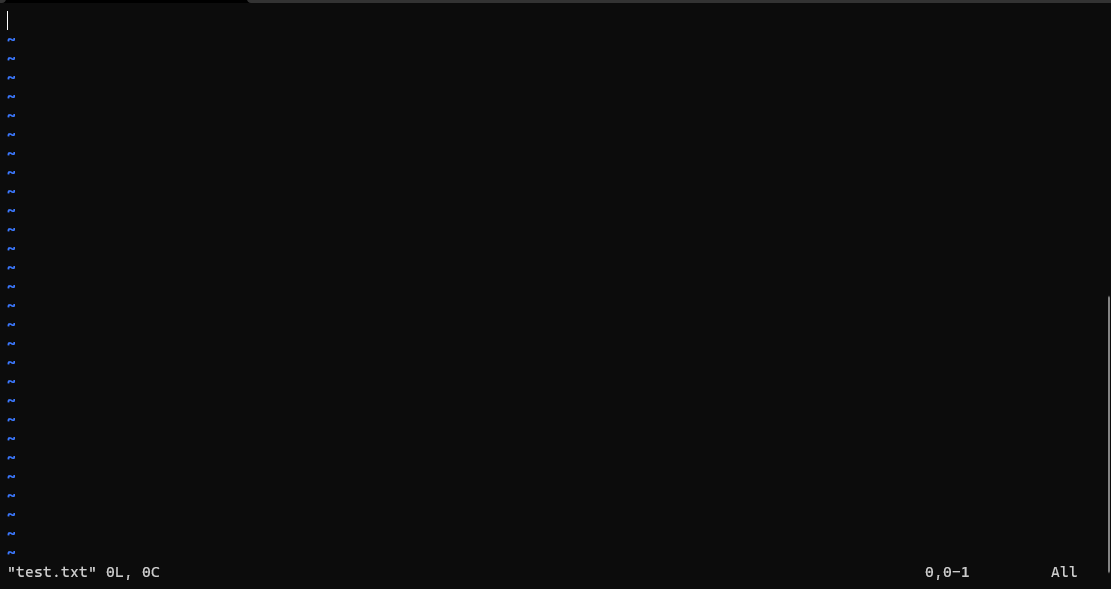
\includegraphics[width=0.8\linewidth]{chap3/images/vim.png}
        \caption{vim 에디터 실행 화면}
    \end{center}
\end{figure}

그런데 이 상태에서 무언가를 입력하려 하면 아마 파일이 수정되지 않을 것이다.\\
왜냐하면 vim 에디터는 수정 모드가 아니라면 파일의 내용을 수정할 수 없기 때문이다.\\
vim 에디터에서 수정모드로 변환하는 방법은 간단하다. i를 입력하면 수정모드로 변환되며, 만약 수정모드를 다시 끄고 싶다면 ESC 키를 누르면 수정모드가 종료된다.\\
수정모드가 아닌 상태에서는 여러 가지 단축키와 커맨드를 통해 여러 기능을 사용할 수 있는데, 이 문서에서는 자주 사용하는 기능의 단축키만을 다룰 것이다. 아래 단축키들을 자주 사용하므로 미리 숙지해놓자.\\

\subsubsection{이동}
\paragraph{기본 이동}
\begin{itemize}[$\bullet$]
    \item h,j,k,l : 좌,하,상,우 커서 이동
    \item - : 줄의 처음 위치로 이동
    \item gg : 맨 위로 커서 이동
    \item Shift + g : 맨 아래로 커서 이동
\end{itemize}
\paragraph{단어 단위로 이동}
\begin{itemize}[$\bullet$]
    \item w : 단어의 시작 위치로 커서 이동 (forward 방향)
        \begin{itemize}[Ex)]
            \item 3w : 세 단어 앞으로 커서 이동
        \end{itemize}
    \item e : 단어의 마지막 위치로 커서 이동 (forward 방향)
    \item b : 단어의 시작 위치로 커서 이동 (backward 방향)
    \item ge : 단어의 마지막 위치로 커서 이동 (backward 방향)
\end{itemize}
\paragraph{한 문장 내에서의 이동}
\begin{itemize}[$\bullet$]
    \item \^ : 문장 맨 앞으로 커서 이동
    \item \$ : 문장 맨 뒤로 커서 이동
\end{itemize}
\paragraph{대략적인 위치로 이동}
\begin{itemize}[$\bullet$]
    \item Shift + h : 현재 보이는 페이지를 기준으로 맨 위로 커서 이동
    \item Shift + m : 현재 보이는 페이지를 기준으로 중간 라인으로 커서 이동
    \item Shift + l : 현재 보이는 페이지를 기준으로 가장 아래로 커서 이동
\end{itemize}
\paragraph{페이지 이동}
\begin{itemize}[$\bullet$]
    \item Ctrl + f : 다음 페이지의 첫 줄로 커서 이동
    \item Ctrl + b : 다음 페이지의 마지막 줄로 커서 이동
    \item Ctrl + d : 페이지의 절반 크기만큼 아래로 커서 이동
    \item Ctrl + u : 페이지의 절반 크기만큼 위로 커서 이동
\end{itemize}
\paragraph{원하는 줄 번호로 한번에 이동}
\begin{itemize}[$\bullet$]
    \item :[number] : [number]행으로 이동
        \begin{itemize}[Ex)]
            \item :3 : 3번째 줄로 이동. 줄 번호는 1부터 시작한다.
        \end{itemize}
\end{itemize}
\paragraph{\{\} 기준으로 이동}
\begin{itemize}[$\bullet$]
    \item ]] : \{로 커서 이동 (forward 방향)
        \begin{itemize}[$\circ$]
            \item 없으면 페이지의 맨 아래로 커서 이동
            \item \{은 가장 상위의 블록을 감싸고 있는 문자만 찾는다.
        \end{itemize}
    \item[$\bullet$] [[ : \{로 커서 이동 (backward 방향)
    \item ][ : \}로 커서 이동 (forward 방향)
        \begin{itemize}[$\circ$]
            \item 없으면 페이지의 맨 아래로 커서 이동
            \item \}은 가장 상위의 블록을 감싸고 있는 문자만 찾는다.
        \end{itemize}
    \item[$\bullet$] [] : \}로 커서 이동 (backward 방향)
    \item \% : \{\}나 ()에서 현재 괄호의 짝으로 커서 이동
\end{itemize}

\subsubsection{편집}
\paragraph{삽입 관련 단축키}
\begin{itemize}[$\bullet$]
    \item i : 현재 커서가 위치한 문자의 앞에 insert 하기
    \item I : 현재 커서가 위치한 줄 맨 앞에 insert 하기
    \item a : 현재 커서가 위치한 문자의 뒤에 insert 하기
    \item A : 현재 커서가 위치한 줄 맨 뒤에 insert 하기
    \item O : 현재 커서가 위치한 줄 바로 윗줄에 insert 하기
    \item o : 현재 커서가 위치한 줄 바로 아랫줄에 insert 하기
\end{itemize}
\paragraph{삭제/잘라내기 및 수정 관련 단축키}
\begin{itemize}[$\bullet$]
    \item dd : 커서가 위치한 줄 잘라내기
    \item dw : 커서가 위치한 곳부터 단어의 마지막까지 잘라내기
    \item Shift + d : 커서가 위치한 곳부터 줄의 끝까지 잘라내기
    \item x : 커서가 위치한 문자 잘라내기
    \item Shift + x : 커서가 위치한 문자 바로 앞에 있는 문자 잘라내기
    \item s : 커서가 위치한 문자 잘라내고 insert 하기
    \item cc 또는 Shift + s : 커서가 위치한 줄 전체 잘라내고 insert 하기
    \item cw : 커서가 위치한 곳부터 단어의 마지막까지 잘라내고 insert 하기
    \item Shift + c : 현재 커서의 위치부터 줄의 끝까지 잘라내고 insert 하기
    \item r + [변경할 문자] : 커서가 위치한 문자 하나 수정하기
        \begin{itemize}[Ex)]
            \item 4rx : 현재 커서 이후 4개의 글자를 x로 수정한다.
        \end{itemize}
\end{itemize}
\paragraph{복사/붙여넣기 관련 단축키}
\begin{itemize}[$\bullet$]
    \item yl : 현재 커서가 위치한 문자 하나만 복사하기
        \begin{itemize}[Ex)]
            \item 3yl : 현재 커서 이후 3개의 문자를 복사한다.
        \end{itemize}
    \item yy : 현재 커서가 위치한 줄 복사하기
    \item yw : 현재 커서의 위치부터 단어가 끝나는 위치까지 복사하기
    \item y : 블럭 단위로 체크한 내용(비주얼 모드 이용) 복사하기 - 한 문자만 복사 X
        \begin{itemize}[Ex)]
            \item[Ex)] [number] + y : 커서가 위치한 줄부터 [number]만큼의 줄 복사하기
            \item y\$ : 커서가 위치한 곳부터 줄의 마지막까지 복사하기
        \end{itemize}
    \item p : 복사한 것을 붙여넣기. 단어를 복사한 경우 커서가 위치한 곳에 붙여넣고, 행 단위를 복사한 경우 커서가 위치한 줄 다음 줄에 붙여넣는다.
    \item Shift + p : 복사한 것을 앞에 붙여넣기. 단어를 복사한 경우 커서가 위치한 곳 앞에 붙여넣고, 행 단위를 복사한 경우 커서가 위치한 줄 바로 윗줄에 붙여넣는다.
    \item[$\bullet$] [number] + p : [number] 만큼 붙여넣기를 반복.
\end{itemize}

이외에도 다양한 단축키가 있으니, 위 목록에 없는 단축키를 안다면 추후 추가 바람.

\subsection{Pipeline}
파이프라인을 통해 출력값에서 원하는 문자열을 확인할 수 있다. 보통 아래와 같이 |와 grep을 이용해 사용한다. 아래의 경우 file2.txt를 출력하는데, 그중 "abc"가 포함된 부분을 찾는 것이다.
    \begin{lstlisting}
    $ cat file2.txt | grep abc
    \end{lstlisting}
